\UC{Registrazione} \label{AccessoPiattaforma}
\label{registrazione}

\begin{figure}[H]
	\centering
	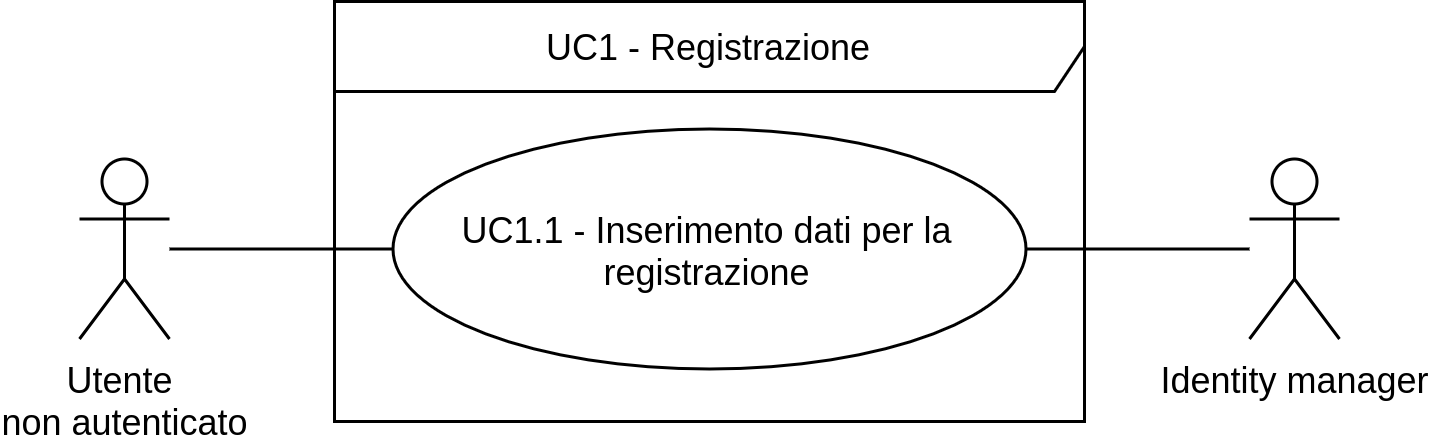
\includegraphics[scale=1]{Immagini/DiagrammiUC/AccessoAllaPiattaforma/Registrazione.png}
	\caption{Diagramma di \actualUC: Registrazione}
	\label{fig:registrazione}
\end{figure}

L'utente non autenticato che non dispone di credenziali può registrarsi e accedere come acquirente nella piattaforma compilando alcuni campi obbligatori per poter procedere.
\begin{itemize}
	\item \textbf{Attori primari:} utente non autenticato;
	\item \textbf{Attori secondari:} \glo{identity manager};
	\item \textbf{Precondizione:} l'utente non è ancora presente nella piattaforma;
	\item \textbf{Postcondizione:} l'utente è registrato con un account acquirente ed è autenticato come tale sulla piattaforma;
	\item \textbf{Scenario principale:}
	\begin{itemize}
		\item L'utente accede al sistema;
		\item L'utente non autenticato si trova nella schermata di registrazione;
		\item (UC\ref{registrazione.modulo}) - Inserimento dati per la registrazione;
		\item L'utente non autenticato conferma il proprio indirizzo e-mail inserito;
		\item L'utente possiede un account presso il sistema.
	\end{itemize}
	\item \textbf{Estensioni:}
	\begin{enumerate}[label=\lett]
		\item L'utente inserisce un indirizzo e-mail e l'identity manager segnala che è già presente nella piattaforma
		\begin{itemize}
			\item L'utente non viene registrato presso il sistema;
			\item (UC\ref{estensione:registrazione-con-email-non-esistente}) - Visualizzazione messaggio di errore in caso di registrazione con un'e-mail già utilizzata nella piattaforma;
			\item Viene fornita all'utente la possibilità di modificare il proprio indirizzo e-mail inserito.
		\end{itemize}
		\item L'utente compila i campi dati per la password e la conferma della stessa con due password diverse, in questo caso:
		\begin{itemize}
			\item L'utente non viene registrato presso il sistema;
			\item L'identity manager segnala che le due password inserite non coincidono;
			\item (UC\ref{estensione:password-conferma-diverse}) - Visualizzazione messaggio di errore in caso di password e password di conferma diverse;
			\item L'utente può modificare le password inserite.
		\end{itemize}
	\end{enumerate}
\end{itemize}

\subUC{Inserimento dati per la registrazione}
\label{registrazione.modulo}

\begin{figure}[H]
	\centering
	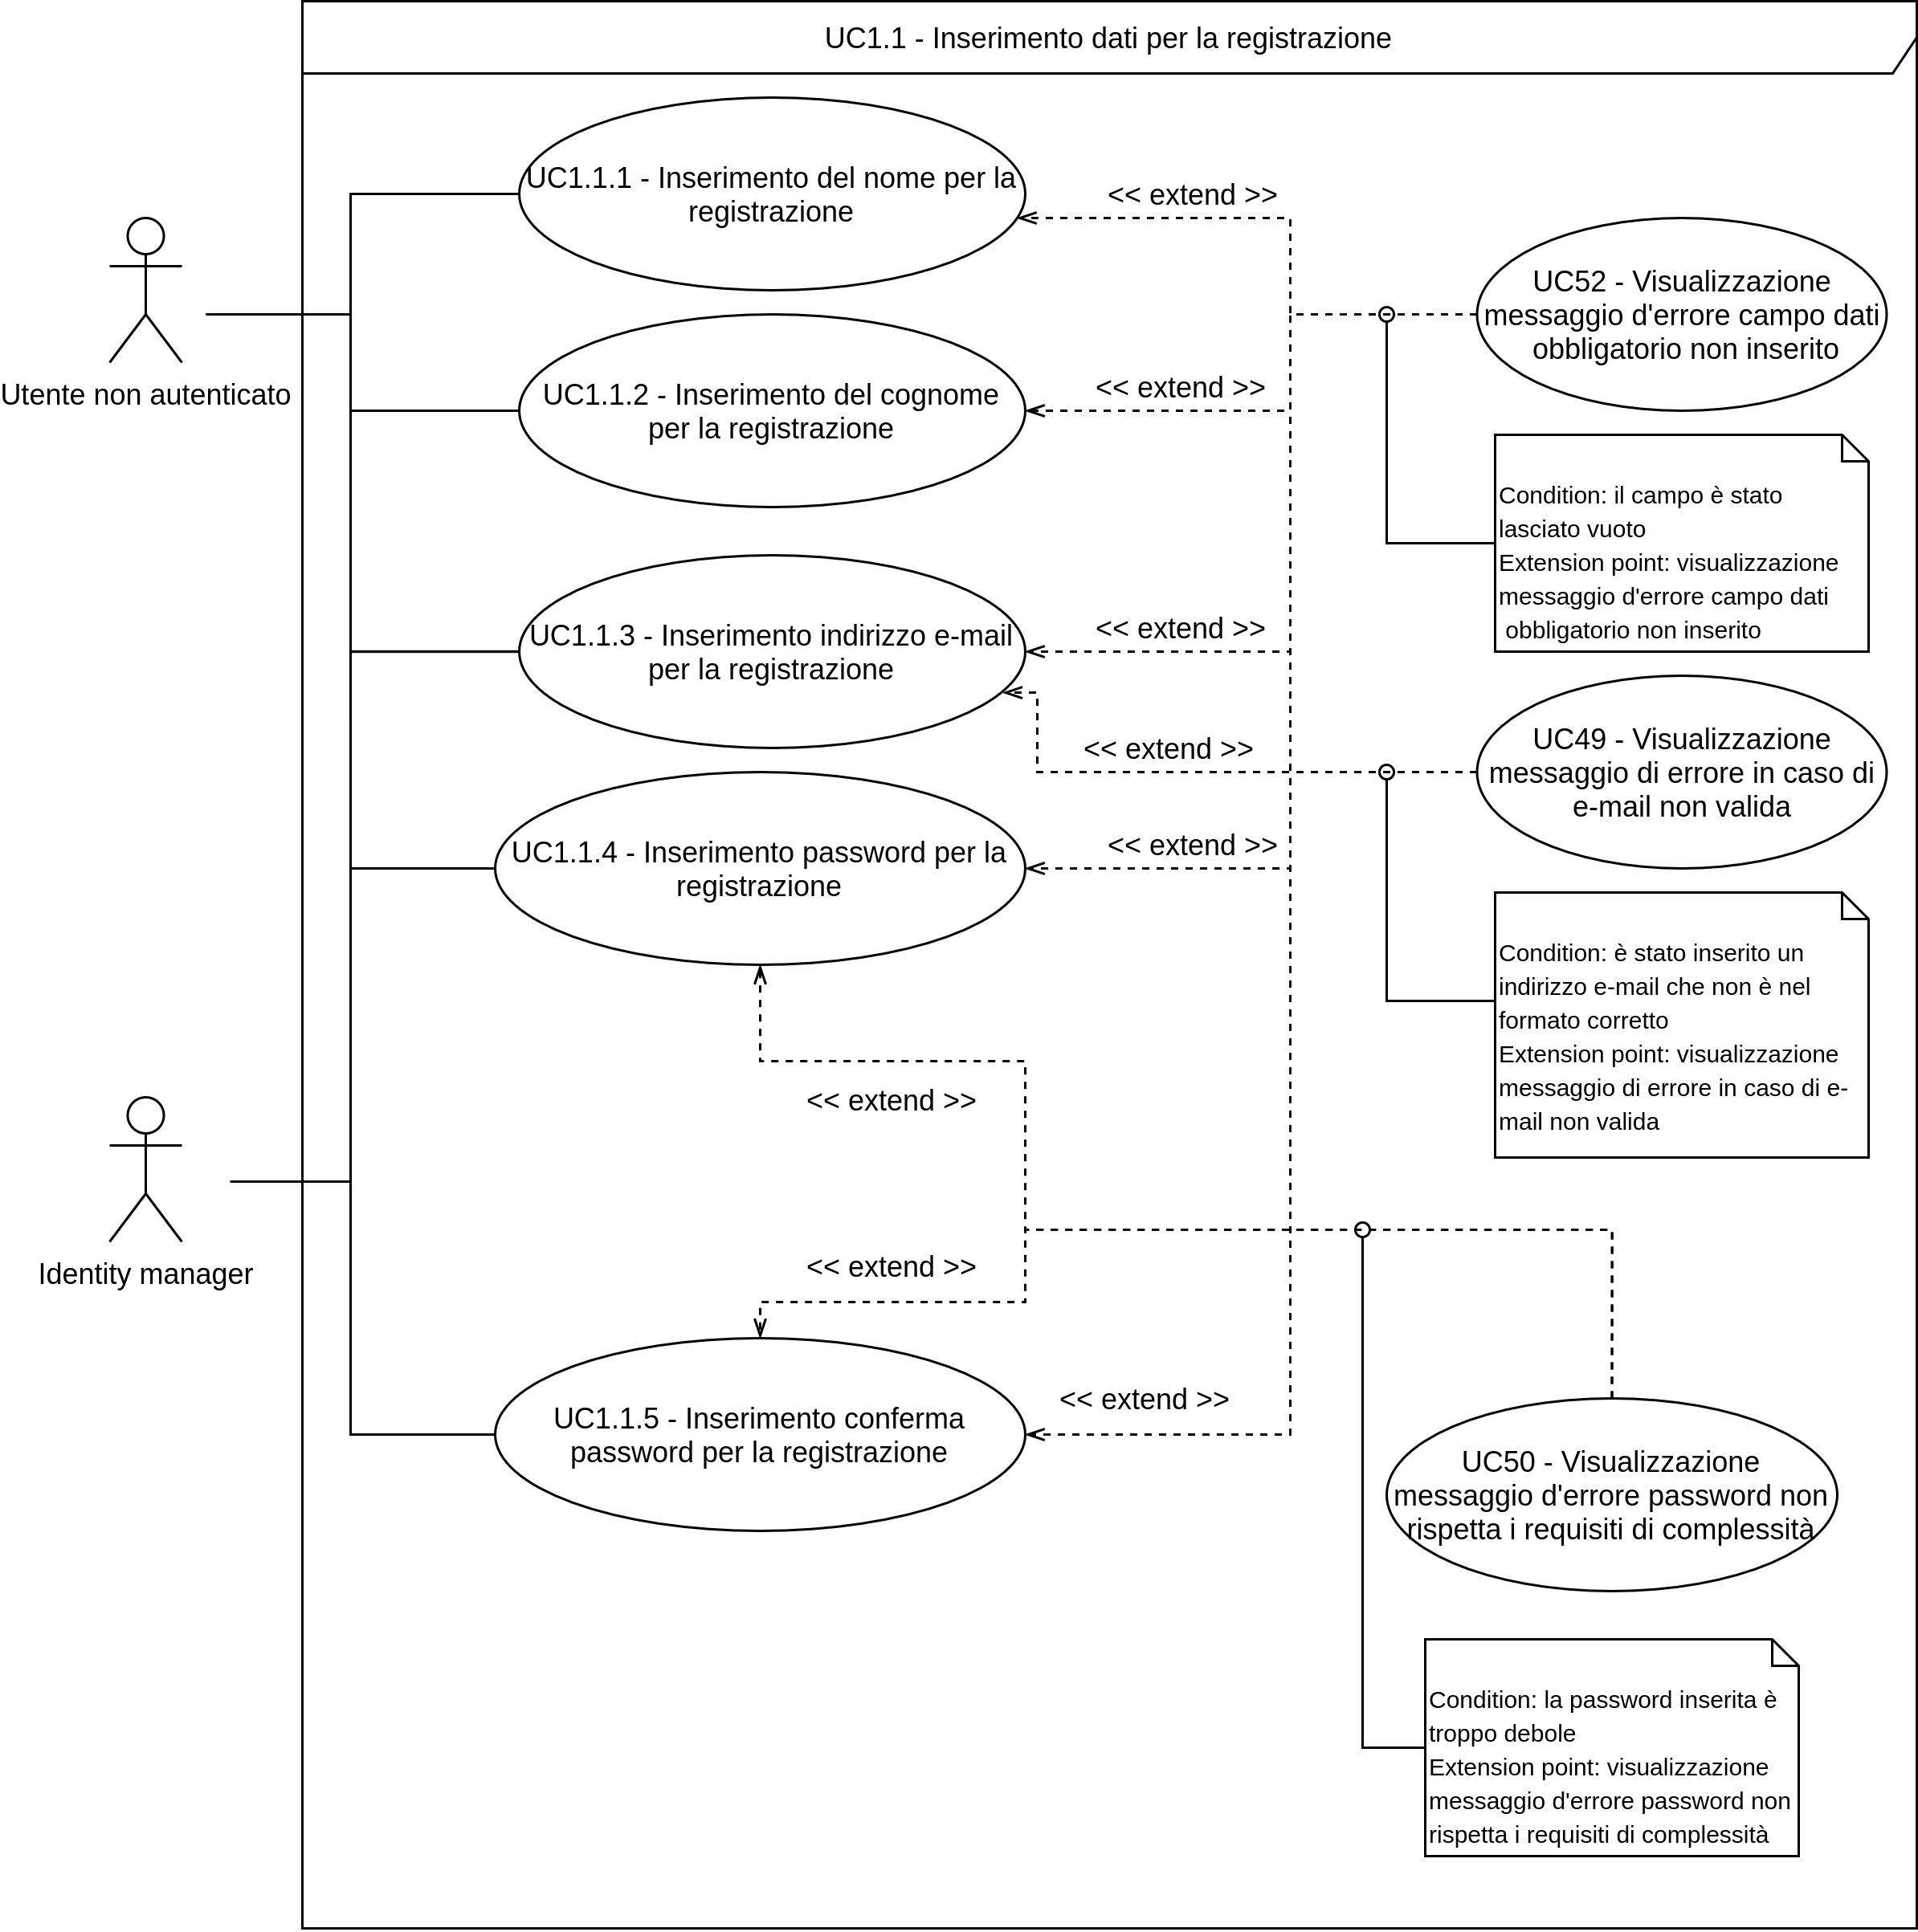
\includegraphics[scale=0.6]{Immagini/DiagrammiUC/AccessoAllaPiattaforma/InserimentoDatiRegistrazione.png}
	\caption{Diagramma di \actualSubUC: Inserimento dati per la registrazione}
	\label{fig:registrazione.modulo}
\end{figure}

L'utente compila il modulo per proseguire con la registrazione presso la piattaforma.
\begin{itemize}
	\item \textbf{Attori primari:} utente non autenticato;
	\item \textbf{Attori secondari:} identity manager;
	\item \textbf{Precondizione:} l'utente non è autenticato e si trova all'interno della schermata di registrazione;
	\item \textbf{Postcondizione:} l'utente ha compilato il modulo e può procedere con la registrazione;
	\item \textbf{Scenario principale:} l'utente non autenticato compila i campi nel seguente modo:
	\begin{itemize}
		\item (UC\ref{registrazione.modulo.nome}) - Inserimento nome per la registrazione;
		\item (UC\ref{registrazione.modulo.cognome}) - Inserimento cognome per la registrazione;
		\item (UC\ref{registrazione.modulo.email}) - Inserimento indirizzo e-mail per la registrazione;
		\item (UC\ref{registrazione.modulo.password}) - Inserimento password per la registrazione;
		\item (UC\ref{registrazione.modulo.conferma-password}) - Inserimento conferma password per la registrazione.
	\end{itemize}
\end{itemize}

\subSubUC{Inserimento del nome per la registrazione}
\label{registrazione.modulo.nome}

L'utente non autenticato inserisce il nome con il quale vuole registrarsi.
\begin{itemize}
	\item \textbf{Attori primari:} utente non autenticato;
	\item \textbf{Attori secondari:} identity manager;
	\item \textbf{Precondizione:} l'utente non è autenticato;
	\item \textbf{Postcondizione:} l'utente ha inserito il proprio nome;
	\item \textbf{Scenario principale:} l'utente non autenticato inserisce il proprio nome per la registrazione;
	\item \textbf{Estensioni:}
	\begin{enumerate}[label=\lett]
		\item L'utente non inserisce il nome e l'identity manager controlla il campo dati per il nome che non risulta compilato, in questo caso:
		\begin{itemize}
			\item (UC\ref{estensione:campo-obbligatorio-non-inserito}) - Viene mostrato un messaggio d'errore campo dati obbligatorio non inserito;
			\item Viene fornita all'utente la possibilità di inserire un nome.
		\end{itemize}
	\end{enumerate} 
\end{itemize}

\subSubUC{Inserimento del cognome per la registrazione}
\label{registrazione.modulo.cognome}

L'utente non autenticato inserisce il cognome con il quale vuole registrarsi.
\begin{itemize}
	\item \textbf{Attori primari:} utente non autenticato;
	\item \textbf{Attori secondari:} identity manager;
	\item \textbf{Precondizione:} l'utente non è autenticato;
	\item \textbf{Postcondizione:} l'utente ha inserito il proprio cognome;
	\item \textbf{Scenario principale:} l'utente non autenticato inserisce il proprio cognome per la registrazione;
	\item \textbf{Estensioni:}
	\begin{enumerate}[label=\lett]
		\item L'utente non inserisce il cognome e l'identity manager controlla il campo dati per il cognome che non risulta compilato, in questo caso:
		\begin{itemize}
			\item (UC\ref{estensione:campo-obbligatorio-non-inserito}) - Viene mostrato un messaggio d'errore campo dati obbligatorio non inserito;
			\item Viene fornita all'utente la possibilità di inserire un cognome.
		\end{itemize}
	\end{enumerate}
\end{itemize}

\subSubUC{Inserimento indirizzo e-mail per la registrazione}
\label{registrazione.modulo.email}

L'utente non autenticato inserisce l'indirizzo e-mail con il quale vuole registrarsi.
\begin{itemize}
	\item \textbf{Attori primari:} utente non autenticato;
	\item \textbf{Attori secondari:} identity manager;
	\item \textbf{Precondizione:} l'utente non autenticato non ha ancora fornito un'e-mail ed ha a disposizione un campo dati dove inserirla;
	\item \textbf{Postcondizione:} l'utente non autenticato ha fornito un indirizzo e-mail valido;
	\item \textbf{Scenario principale:} l'utente non autenticato inserisce il proprio indirizzo e-mail per procedere con la registrazione;
	\item \textbf{Estensioni:}
	\begin{enumerate}[label=\lett]
		\item L'utente non inserisce l'e-mail e l'identity manager controlla il campo dati che risulta essere vuoto, in questo caso:
		\begin{itemize}
			\item (UC\ref{estensione:campo-obbligatorio-non-inserito}) - Viene mostrato un messaggio d'errore campo dati obbligatorio non inserito;
			\item Viene fornita all'utente la possibilità di inserire un indirizzo e-mail.
		\end{itemize}
		\item L'utente non autenticato ha inserito un indirizzo e-mail e l'identity manager segnala che non è nel formato non corretto, in questo caso:
		\begin{itemize}
			\item (UC\ref{estensione:email-non-valida}) - Viene mostrato un messaggio d'errore indirizzo e-mail non rispetta il formato;
			\item Viene fornita all'utente la possibilità di modificare l'indirizzo e-mail inserito.
		\end{itemize}
	\end{enumerate}
\end{itemize}

\subSubUC{Inserimento password per la registrazione}
\label{registrazione.modulo.password}

L'utente non autenticato inserisce la password con la quale vuole registrarsi.
\begin{itemize}
	\item \textbf{Attori primari:} utente non autenticato;
	\item \textbf{Attori secondari:} identity manager;
	\item \textbf{Precondizione:} l'utente non autenticato non ha ancora fornito una password che rispetta i requisiti di complessità ed ha a disposizione un campo dati dove inserirla;
	\item \textbf{Postcondizione:} l'utente ha inserito una password valida;
	\item \textbf{Scenario principale:} l'utente non autenticato inserisce una password che rispetti le condizioni imposte per procedere con la registrazione;
	\item \textbf{Estensioni:}
	\begin{enumerate}[label=\lett]
		\item L'utente non inserisce la password e l'identity manager controlla il campo dati che risulta essere vuoto, in questo caso:
		\begin{itemize}
			\item (UC\ref{estensione:campo-obbligatorio-non-inserito}) - Viene mostrato un messaggio d'errore campo dati obbligatorio non inserito;
			\item Viene fornita all'utente la possibilità di inserire una password.
		\end{itemize}
		\item L'utente non autenticato ha inserito una password e l'identity manager segnala che non è nel formato corretto, in questo caso:
		\begin{itemize}
			\item (UC\ref{estensione:password-non-valida}) - Viene mostrato un messaggio d'errore password non rispetta i requisiti di complessità;
			\item Viene fornita all'utente la possibilità di modificare la password inserita.
		\end{itemize}
	\end{enumerate} 
\end{itemize}

\subSubUC{Inserimento conferma password per la registrazione}
\label{registrazione.modulo.conferma-password}

L'utente non autenticato inserisce la conferma della password con la quale vuole registrarsi.
\begin{itemize}
	\item \textbf{Attori primari:} utente non autenticato;
	\item \textbf{Attori secondari:} identity manager;
	\item \textbf{Precondizione:} l'utente non autenticato non ha ancora fornito una password che rispetta i requisiti di complessità ed ha a disposizione un campo dati dove inserirla;
	\item \textbf{Postcondizione:} l'utente ha inserito la conferma della password ed è valida;
	\item \textbf{Scenario principale:} l'utente non autenticato inserisce una password che rispetti le condizioni imposte per procedere con la registrazione;
	\item \textbf{Estensioni:} 
	\begin{enumerate}[label=\lett]
		\item L'utente non inserisce la conferma password e l'identity manager controlla il campo dati che risulta essere vuoto, in questo caso:
		\begin{itemize}
			\item (UC\ref{estensione:campo-obbligatorio-non-inserito}) - Viene mostrato un messaggio d'errore campo dati obbligatorio non inserito;
			\item Viene fornita all'utente la possibilità di inserire una password.
		\end{itemize}
		\item L'utente non autenticato ha inserito una password e l'identity manager segnala che non è nel formato corretto, in questo caso:
		\begin{itemize}
			\item (UC\ref{estensione:password-non-valida}) - Viene mostrato un messaggio d'errore password non rispetta i requisiti di complessità;
			\item Viene fornita all'utente la possibilità di modificare la password inserita.
		\end{itemize}
	\end{enumerate} 
\end{itemize}

\UC{Autenticazione nella piattaforma}
\label{autenticazione-piattaforma}

\begin{figure}[H]
    \centering
    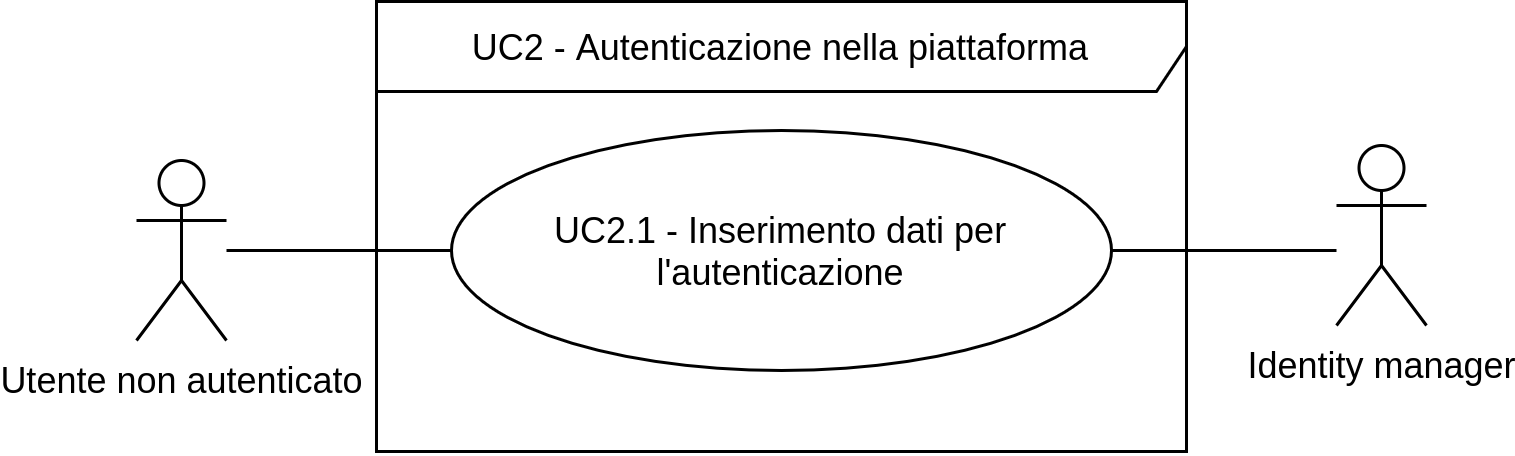
\includegraphics[scale=1]{Immagini/DiagrammiUC/AccessoAllaPiattaforma/AutenticazionePiattaforma.png}
    \caption{Diagramma di \actualUC: Autenticazione nella piattaforma} 
    \label{fig:autenticazione-piattaforma}
\end{figure}

L'utente non autenticato che dispone di credenziali può accedere nella piattaforma usando l'e-mail e la password.
\begin{itemize}
    \item \textbf{Attori primari:} utente non autenticato;
    \item \textbf{Attori secondari:} identity manager;
    \item \textbf{Precondizione:} l'utente non autenticato dispone di credenziali;
    \item \textbf{Postcondizione:} l'utente è autenticato come utente autenticato;
    \item \textbf{Scenario principale:}
    \begin{itemize}
    	\item L'utente accede al sistema;
    	\item L'utente non autenticato si trova nella schermata di login;
    	\item (UC\ref{autenticazione-piattaforma.modulo}) - Inserimento dati per l'autenticazione;% Inserisce le credenziali per accedere alla piattaforma
    	\item L'utente richiede l'autenticazione;
    	\item L'utente è autenticato come utente autenticato;
    \end{itemize}
	\item \textbf{Estensioni:}
	\begin{enumerate}[label=\lett]
		\item L'utente compila i campi dati con delle credenziali, richiede l'autenticazione e l'identity manager segnala che le credenziali fornite non appartengono alla piattaforma
		\begin{itemize}
			\item L'utente non viene autenticato presso il sistema;
			\item (UC\ref{estensione:credenziali-non-presenti}) - Viene visualizzato un messaggio di errore credenziali non presenti nella piattaforma;
			\item Viene fornita all'utente la possibilità di modificare i valori inseriti nel modulo di autenticazione.
		\end{itemize}
	\end{enumerate} 
\end{itemize}

\subUC{Inserimento dati per l'autenticazione}
\label{autenticazione-piattaforma.modulo}

\begin{figure}[H]
	\centering
	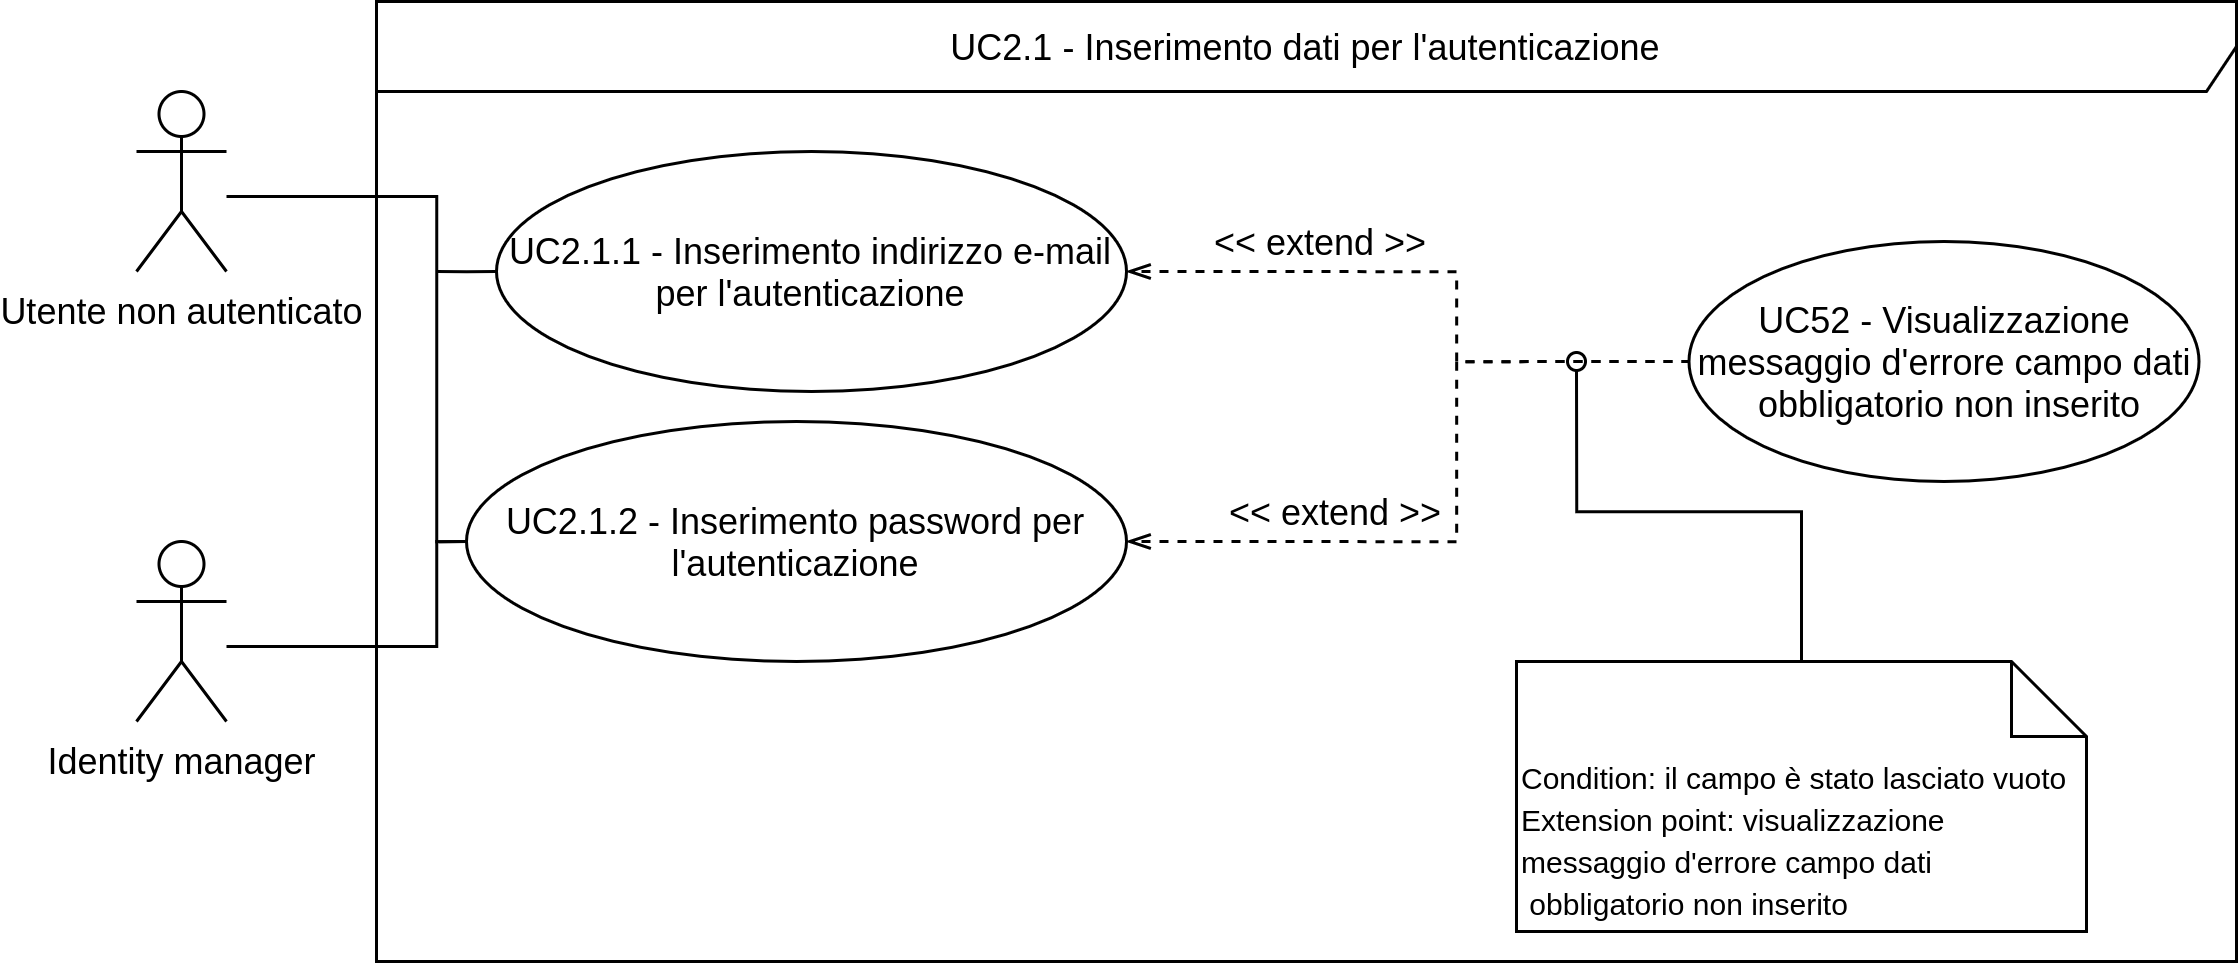
\includegraphics[scale=0.8]{Immagini/DiagrammiUC/AccessoAllaPiattaforma/InserimentoDatiAutenticazione.png}
	\caption{Diagramma di \actualSubUC: Inserimento dati per l'autenticazione}
	\label{fig:autenticazione-piattaforma.modulo}
\end{figure}

L'utente compila il modulo per proseguire con l'autenticazione presso la piattaforma.
\begin{itemize}
	\item \textbf{Attori primari:} utente non autenticato;
	\item \textbf{Attori secondari:} identity manager;
	\item \textbf{Precondizione:} l'utente non è autenticato e si trova all'interno della schermata di login;
	\item \textbf{Postcondizione:} l'utente ha compilato il modulo e può procedere con l'autenticazione;
	\item \textbf{Scenario principale:} l'utente non autenticato compila i campi nel seguente modo:
	\begin{itemize}
		\item (UC\ref{autenticazione-piattaforma.modulo.email}) - Inserimento indirizzo e-mail per l'autenticazione;
		\item (UC\ref{autenticazione-piattaforma.modulo.password}) - Inserimento password per l'autenticazione.
	\end{itemize}
\end{itemize}

\subSubUC{Inserimento indirizzo e-mail per l'autenticazione}
\label{autenticazione-piattaforma.modulo.email}

L'utente non autenticato inserisce l'indirizzo e-mail collegato al proprio account.
\begin{itemize}
	\item \textbf{Attori primari:} utente non autenticato;
	\item \textbf{Attori secondari:} identity manager;
	\item \textbf{Precondizione:} l'utente non autenticato possiede delle credenziali d'accesso e si trova nella schermata di login;
	\item \textbf{Postcondizione:}  l'utente ha inserito il proprio indirizzo e-mail;
	\item \textbf{Scenario principale:} l'utente non autenticato inserisce il proprio indirizzo e-mail per procedere con l'autenticazione;
	\item \textbf{Estensioni:}
	\begin{enumerate}[label=\lett]
		\item L'utente non inserisce l'e-mail e l'identity manager controlla il campo dati che risulta essere vuoto, in questo caso:
		\begin{itemize}
			\item (UC\ref{estensione:campo-obbligatorio-non-inserito}) - Viene mostrato un messaggio d'errore campo dati obbligatorio non inserito;
			\item Viene fornita all'utente la possibilità di inserire un indirizzo e-mail.
		\end{itemize}
	\end{enumerate}
\end{itemize}

\subSubUC{Inserimento password per l'autenticazione}
\label{autenticazione-piattaforma.modulo.password}

L'utente non autenticato inserisce la password collegata al proprio account.
\begin{itemize}
	\item \textbf{Attori primari:} utente non autenticato;
	\item \textbf{Attori secondari:} identity manager;
	\item \textbf{Precondizione:} l'utente non autenticato possiede delle credenziali d'accesso e si trova nella schermata di login;
	\item \textbf{Postcondizione:} l'utente ha inserito la propria password;
	\item \textbf{Scenario principale:} l'utente non autenticato inserisce la propria password per procedere con l'autenticazione;
	\item \textbf{Estensioni:} 
	\begin{enumerate}[label=\lett]
		\item L'utente non inserisce la password e l'identity manager controlla il campo dati che risulta essere vuoto, in questo caso:
		\begin{itemize}
			\item (UC\ref{estensione:campo-obbligatorio-non-inserito}) - Viene mostrato un messaggio d'errore campo dati obbligatorio non inserito;
			\item Viene fornita all'utente la possibilità di inserire una password.
		\end{itemize}
	\end{enumerate}
\end{itemize}

\UC{Password dimenticata}
\label{password-dimenticata}

\begin{figure}[H]
    \centering
    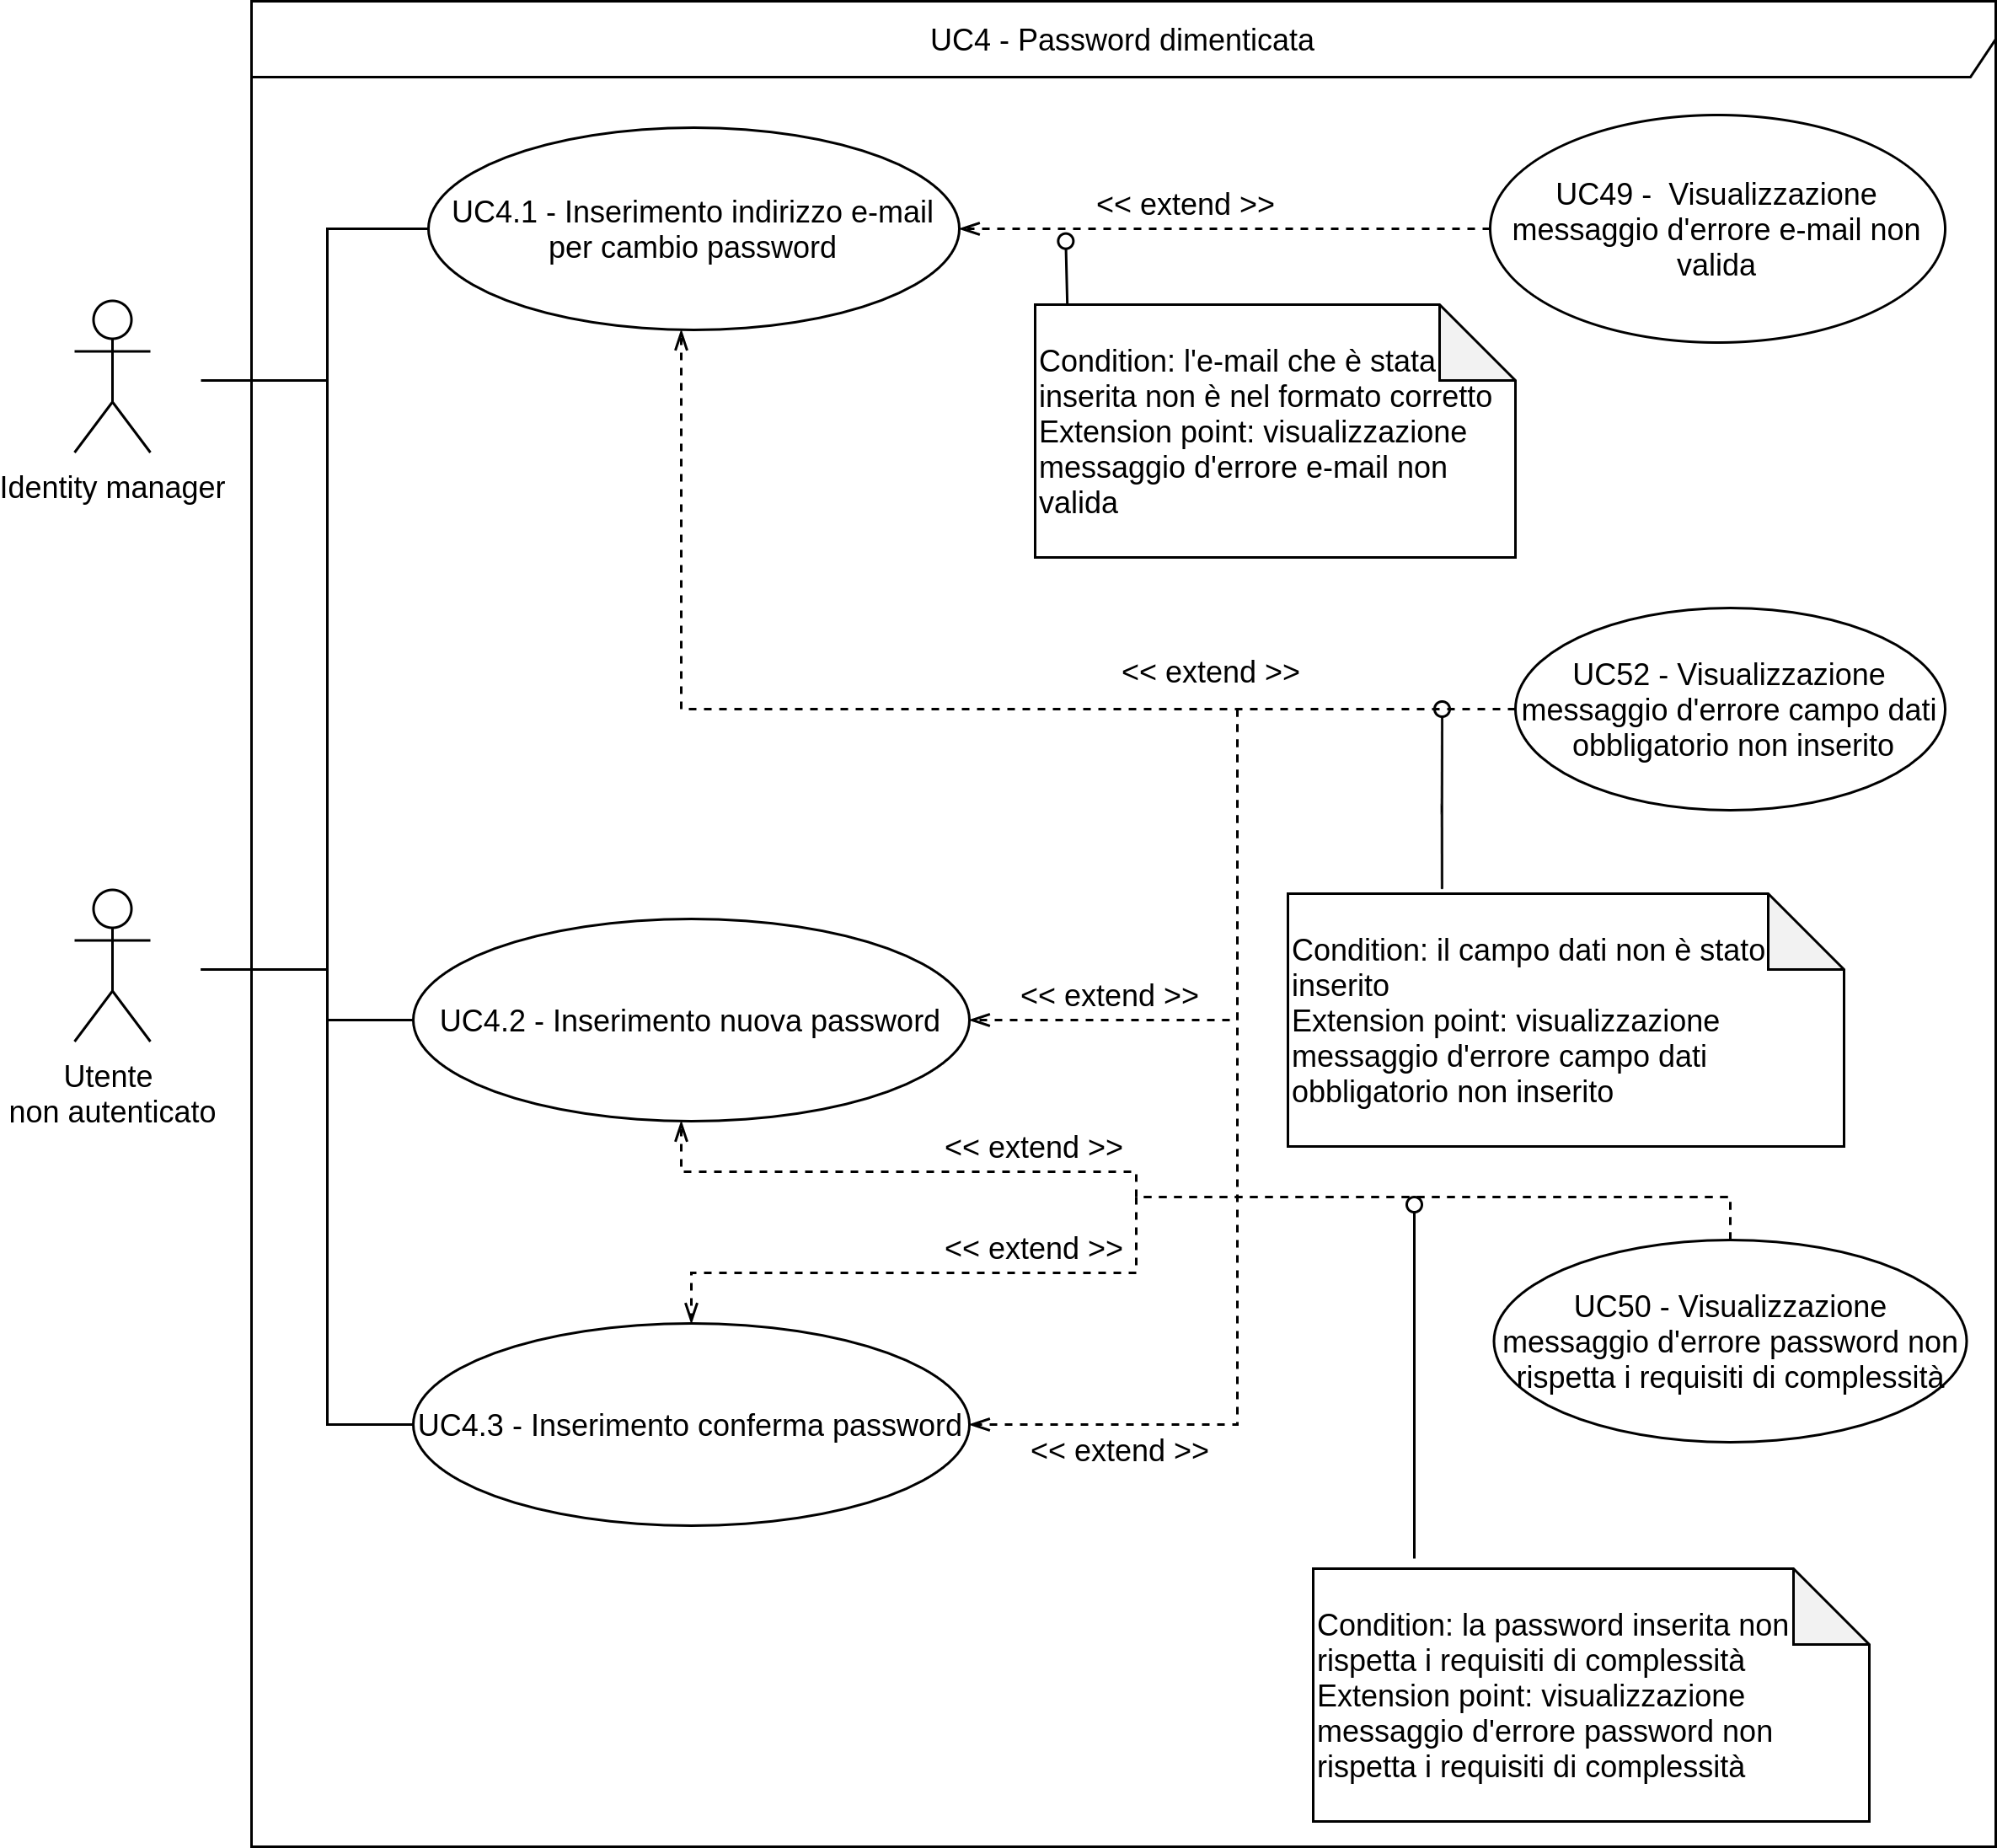
\includegraphics[scale=0.5]{Immagini/DiagrammiUC/AccessoAllaPiattaforma/PasswordDimenticata.png}
    \caption{Diagramma di \actualUC: Password dimenticata} 
    \label{fig:password-dimenticata}
\end{figure}

L'utente che dispone di credenziali si è dimenticato la propria password e la vuole cambiare.
\begin{itemize}
    \item \textbf{Attori primari:} utente non autenticato;
    \item \textbf{Autori secondari:} identity manager;
    \item \textbf{Precondizione:} l'utente non autenticato che dispone di credenziali si trova nella schermata per cambiare la password;
    \item \textbf{Postcondizione:} l'utente è autenticato e ha cambiato la password con cui poter effettuare l'accesso alla piattaforma;
    \item \textbf{Scenario principale:} l'utente che dispone di credenziali si è dimenticato la propria password e per cambiarla deve compiere i seguenti passi:
    \begin{itemize}
        \item (UC\ref{password-dimenticata.email}) - Inserimento indirizzo e-mail per cambio password;
        \item Invio link per il cambio della password all'indirizzo e-mail indicato;
        \item Apertura della schermata per il cambio della password;
        \item (UC\ref{password-dimenticata.password}) - Inserimento nuova password;
        \item (UC\ref{password-dimenticata.conferma-password}) - Inserimento conferma nuova password;
        \item L'utente è autenticato e ha cambiato la password.
    \end{itemize}
	\item \textbf{Scenari alternativi:}
	\begin{enumerate}[label=\lett]
		\item Se l'utente non autenticato non seleziona il link per il cambio della password che gli è stato inviato all'indirizzo e-mail indicato entro un tempo limite, allora non sarà più valido e dovrà compiere nuovamente tutta la procedura per il cambio della password. 
	\end{enumerate}
	\item \textbf{Estensioni:}
	\begin{enumerate}[label=\lett]
		\item L'utente non autenticato inserisce un indirizzo e-mail e l'identity manager segnala che l'indirizzo e-mail non è presente nella piattaforma, in questo caso:
		\begin{itemize}
			\item (UC\ref{estensione:email-non-esistente}) - Viene visualizzato un messaggio di errore indirizzo e-mail non registrato nella piattaforma;
			\item L'utente rimane non autenticato e alla schermata per cambiare la password.
		\end{itemize}
		\item L'utente non autenticato non inserisce la stessa password nei campi di password e conferma password e l'identity manager lo segnala. In questo caso:
		\begin{itemize}
			\item (UC\ref{estensione:password-conferma-diverse}) - Visualizzazione messaggio di errore in caso di password e password di conferma diverse;
			\item L'utente può modificare le password inserite.
		\end{itemize}
	\end{enumerate}
\end{itemize}

\subUC{Inserimento indirizzo e-mail per cambio password}
\label{password-dimenticata.email}

L'utente che dispone di credenziali si è dimenticato la propria password e inserisce la propria e-mail per poterla cambiare.
\begin{itemize}
    \item \textbf{Attori primari:} utente non autenticato;
    \item \textbf{Autori secondari:} identity manager;
    \item \textbf{Precondizione:} l'utente non autenticato che dispone di credenziali si trova nella schermata di cambio della password;
    \item \textbf{Postcondizione:} l'utente non autenticato ha inserito l'email collegata al proprio account acquirente;
    \item \textbf{Scenario principale:} l'utente non autenticato che dispone di credenziali si trova nella schermata per cambiare la password e ha inserito l'email collegata al proprio account;
	\item \textbf{Estensioni:}
	\begin{enumerate}[label=\lett]
		\item L'utente non inserisce l'e-mail e l'identity manager controlla il campo dati che risulta essere vuoto, in questo caso:
		\begin{itemize}
			\item (UC\ref{estensione:campo-obbligatorio-non-inserito}) - Viene mostrato un messaggio d'errore campo dati obbligatorio non inserito;
			\item Viene fornita all'utente la possibilità di inserire un indirizzo e-mail.
		\end{itemize}
		\item L'utente non autenticato ha inserito un indirizzo e-mail e l'identity manager segnala che non è nel formato non corretto, in questo caso:
		\begin{itemize}
			\item (UC\ref{estensione:email-non-valida}) - Viene mostrato un messaggio d'errore indirizzo e-mail non rispetta il formato;
			\item Viene fornita all'utente la possibilità di modificare l'indirizzo e-mail inserito.
		\end{itemize}
	\end{enumerate}
\end{itemize}

\subUC{Inserimento nuova password}
\label{password-dimenticata.password}

L'utente che dispone di credenziali si è dimenticato la propria password e inserisce la nuova password con la quale si autenticherà.
\begin{itemize}
	\item \textbf{Attori primari:} utente non autenticato;
	\item \textbf{Attori secondari:} identity manager;
	\item \textbf{Precondizione:} l'utente ha selezionato il link per il cambio della password nell'email ricevuta;
	\item \textbf{Postcondizione:} l'utente ha inserito la nuova password con la quale si autenticherà;
	\item \textbf{Scenario principale:} l'utente ha selezionato il link per il cambio della password nell'email ricevuta ed è stato reindirizzato alla schermata dedicata per questo scopo. A quel punto inserirà la nuova password con la quale vorrà autenticarsi;
	\item \textbf{Estensioni:}
	\begin{enumerate}[label=\lett]
		\item L'utente non inserisce la password e l'identity manager controlla il campo dati che risulta essere vuoto, in questo caso:
		\begin{itemize}
			\item (UC\ref{estensione:campo-obbligatorio-non-inserito}) - Viene mostrato un messaggio d'errore campo dati obbligatorio non inserito;
			\item Viene fornita all'utente la possibilità di inserire una password.
		\end{itemize}
		\item L'utente non autenticato ha inserito una password e l'identity manager segnala che non è nel formato corretto, in questo caso:
		\begin{itemize}
			\item (UC\ref{estensione:password-non-valida}) - Viene mostrato un messaggio d'errore password non rispetta i requisiti di complessità;
			\item Viene fornita all'utente la possibilità di modificare la password inserita.
		\end{itemize}
	\end{enumerate}
\end{itemize}

\subUC{Inserimento conferma nuova password}
\label{password-dimenticata.conferma-password}

L'utente non autenticato che dispone di credenziali si è dimenticato la propria password e inserisce la conferma della nuova password con la quale si autenticherà.
\begin{itemize}
	\item \textbf{Attori primari:} utente non autenticato;
	\item \textbf{Attori secondari:} identity manager;
	\item \textbf{Precondizione:} l'utente non autenticato ha selezionato il link per il cambio della password nell'email ricevuta;
	\item \textbf{Postcondizione:} l'utente non autenticato ha inserito la conferma della nuova password con la quale si autenticherà;
	\item \textbf{Scenario principale:} l'utente ha selezionato il link per il cambio della password nell'email ricevuta ed è stato reindirizzato alla schermata dedicata a questo scopo. A quel punto inserirà la conferma della nuova password con la quale vorrà autenticarsi;
	\item \textbf{Estensioni:}
	\begin{enumerate}[label=\lett]
		\item L'utente non inserisce la conferma della nuova password e l'identity manager controlla il campo dati che risulta essere vuoto, in questo caso:
		\begin{itemize}
			\item (UC\ref{estensione:campo-obbligatorio-non-inserito}) - Viene mostrato un messaggio d'errore campo dati obbligatorio non inserito;
			\item Viene fornita all'utente la possibilità di inserire una password.
		\end{itemize}
		\item L'utente non autenticato ha inserito la conferma della nuova password e l'identity manager segnala che non è nel formato corretto, in questo caso:
		\begin{itemize}
			\item (UC\ref{estensione:password-non-valida}) - Viene mostrato un messaggio d'errore password non rispetta i requisiti di complessità;
			\item Viene fornita all'utente la possibilità di modificare la password inserita.
		\end{itemize}
	\end{enumerate}
\end{itemize}

%%%%%%%%%%%%%%%%%%%%%%%%%%%%%%%%%%%%%%%%%%%%%%%%%%%%%%%%%%%%%%%%%%%%%%%%%%%%%%%%%%%%%%%%%%%%%%%%%%%%%%%%%%%%%%%%%%%%%%%%%%%%%%%%%%%%%%%%%%%%%%%%%%%%%%%%%%%%%%%%%%%%%%%%%%%%%%%%%%%%%%%%%%%%%%%%%%%%% 

\UC{Logout dalla piattaforma}
\label{logout}

L'utente autenticato decide di scollegarsi dalla piattaforma.
\begin{itemize}
    \item \textbf{Attori primari:} utente autenticato;
    \item \textbf{Attori secondari:} identity manager;
    \item \textbf{Precondizione:} l'utente ha eseguito il login precedentemente e vuole scollegarsi dalla piattaforma;
    \item \textbf{Postcondizione:} l'utente autenticato diventa un utente non autenticato;
    \item \textbf{Scenario principale:} l'utente autenticato decide di scollegarsi dalla piattaforma e compie l'azione di scollegamento.
\end{itemize}
